\documentclass[a4paper]{article}
\usepackage{amsmath}
\usepackage{amssymb}
\usepackage{geometry}
\usepackage{enumerate}
\usepackage{natbib}
\usepackage{float}%稳定图片位置
\usepackage{graphicx,subfig}%画图
\usepackage{caption}
\usepackage[english]{babel}
\usepackage{indentfirst}%缩进
\usepackage{enumerate}%加序号
\usepackage{multirow}%合并行
\usepackage{hyperref}
\usepackage{tikz}
\hypersetup{hypertex=true, colorlinks=true, linkcolor=black, anchorcolor=black, citecolor=black}
\title{\Large \textbf{VG441 Problem Set 2}\\
\author{\textbf{Pan, Chongdan ID:516370910121}\\
}
}
\begin{document}
\maketitle
\section{Problem 1}
\quad
Let one day be the unit time, then we get $\lambda=500,K=2250,h=\frac{1}{1460}$
\\\[c=\begin{cases}
    1490 & Q<1200\\
    1220 & 1200\leq Q<2400\\
    1100 & Q\geq 2400
\end{cases}\]
\\When we apply the all-units discount structure:
\\$Q_0^*=\sqrt{\frac{2K\lambda}{hc_0}}=\sqrt{\frac{2\times2250\times500\times1460}{1490}}\approx1484.8$
\\$Q_1^*=\sqrt{\frac{2K\lambda}{hc_1}}=\sqrt{\frac{2\times2250\times500\times1460}{1220}}\approx1640.9$
\\$Q_2^*=\sqrt{\frac{2K\lambda}{hc_2}}=\sqrt{\frac{2\times2250\times500\times1460}{1100}}\approx1728.1$
\\\\Only $Q_0^*$ and $Q_1^*$ are realizable
\\$g_1(Q_1)=500\times1200+\sqrt{2\times2250\times500\times\frac{1}{1460}\times1200}\approx611371.2$
\\\\For the breakpoints
\\$g_1(1200)=500\times1220+\frac{2250\times500}{1200}+\frac{1220\times1200}{2\times1460}\approx611438.9$
\\$g_2(2400)=500\times1100+\frac{2250\times500}{2400}+\frac{1100\times2400}{2\times1460}\approx551372.9$
\\Therefore, it's the optimal order quantity is $Q=2400$ ton, which incurs a purchase cost of 1100\$ and the daily cost is 551372.9\$
\\\\When we apply the incremental discount structure:
\\$\bar{c_1}=1490\times1200-1220\times1200=324000$
\\$\bar{c_2}=1490\times1200+1220\times1200-1100\times2400=612000$
\\$Q_0^*=\sqrt{\frac{2\times2250\times500\times1460}{1490}}=1484.8$
\\$Q_1^*=\sqrt{\frac{2\times(2250+324000)\times500\times1460}{1220}}=19759.3$
\\$Q_2^*=\sqrt{\frac{2\times(2250+612000)\times500\times1460}{1100}}=28553.1$
\\\\Only $Q_2^*$ are realizable
\\$g_2(28553.1)=500\times1100+\frac{612000}{2\times1460}+\sqrt{2\times500\times(2250+612000)\times1100\times\frac{1}{1460}}=571722.2$
\\Therefore, it's the optimal order quantity is $Q=28553.1$ ton, which incurs the daily cost 571722.2\$
\section{Problem 2}
$T=52,K=1100,c=2.4$
\begin{figure}[H]
    \centering
    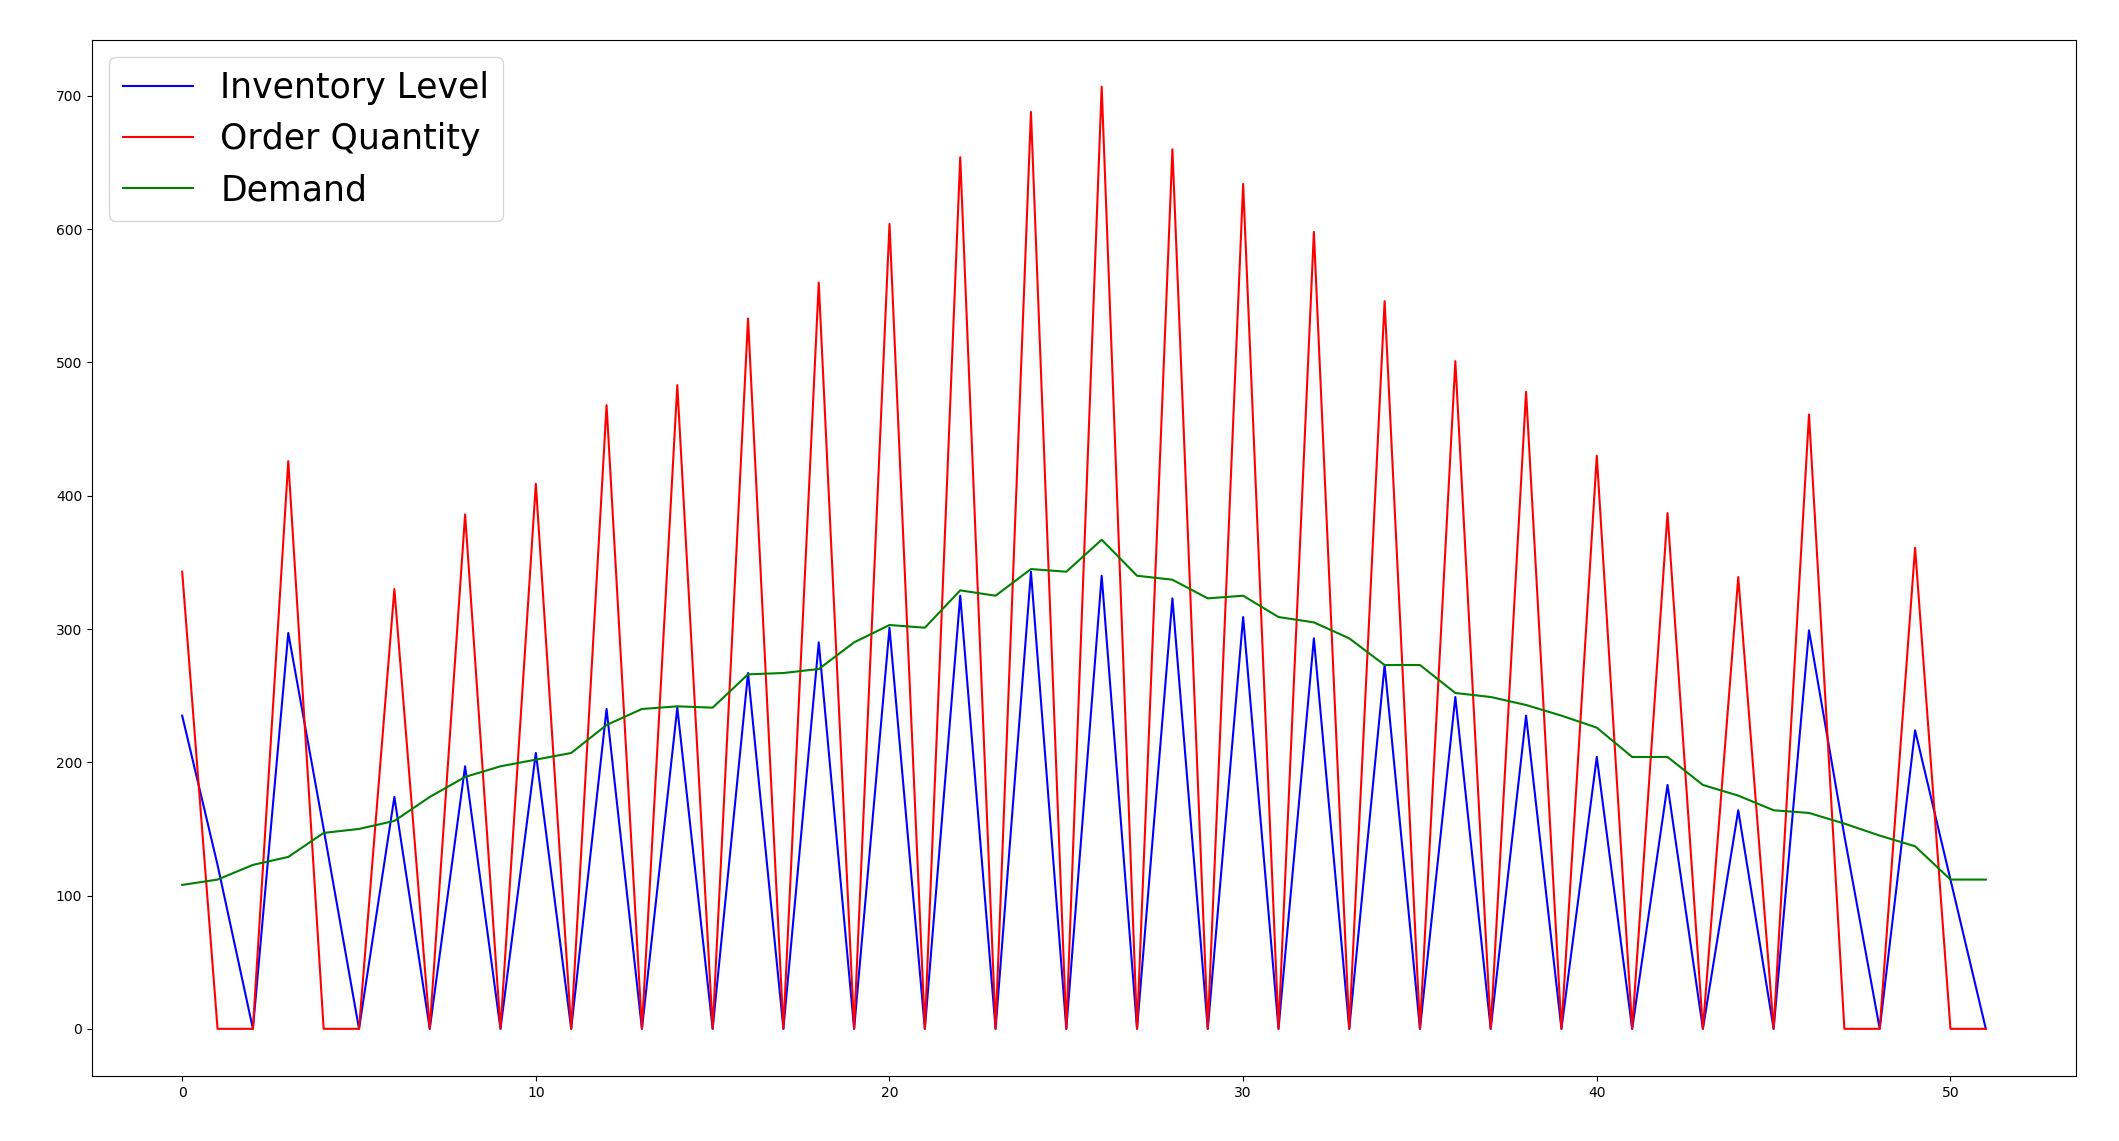
\includegraphics[scale=0.2]{P1.png}
    \caption{Plot of Result}
    \label{P1}
\end{figure}
According to MILP Model computed by guroby package in python, the objective $\sum_{t=1}^T(Ky_t+hx_t)$ is 42583\$, \ref{P1} shows demand, optimal order quantity and corresponding inventory level.
\section{Problem 3}
\textbf{Task 1}
\begin{enumerate}
    \item First, we pick the Path:$s\rightarrow b\rightarrow t$
    \begin{figure}[H]
        \centering
        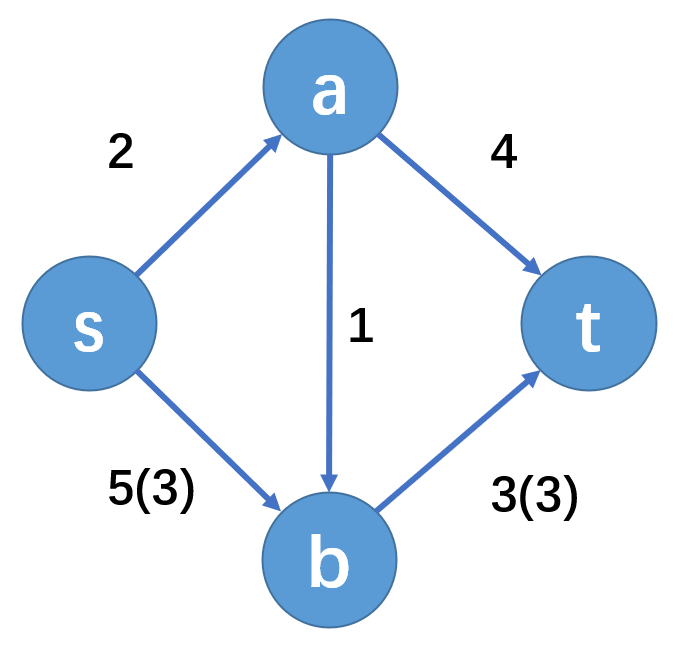
\includegraphics[scale=0.25]{P2.png}
        \caption{Flow Graph of Step 1}
    \end{figure}
    \begin{figure}[H]
        \centering
        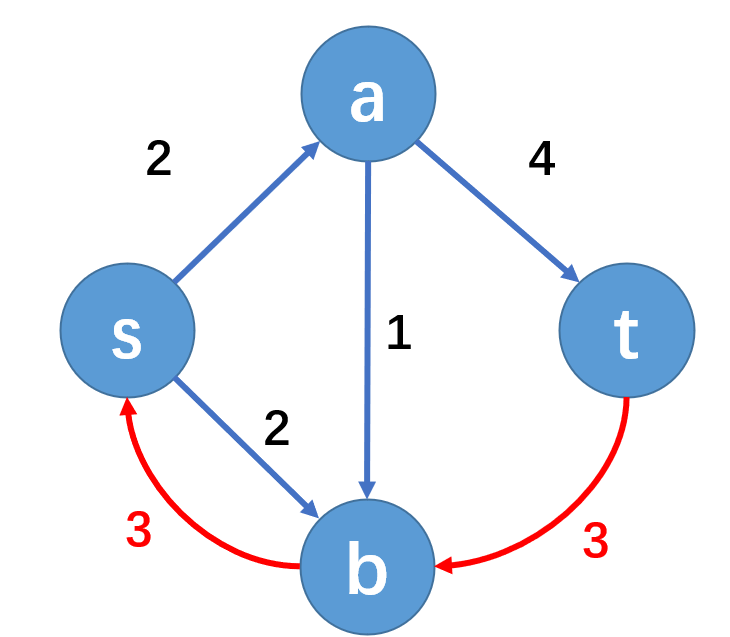
\includegraphics[scale=0.25]{P3.png}
        \caption{Residual Graph of Step 1}
    \end{figure}
    \item Second, we pick the Path:$s\rightarrow a\rightarrow t$
    \begin{figure}[H]
        \centering
        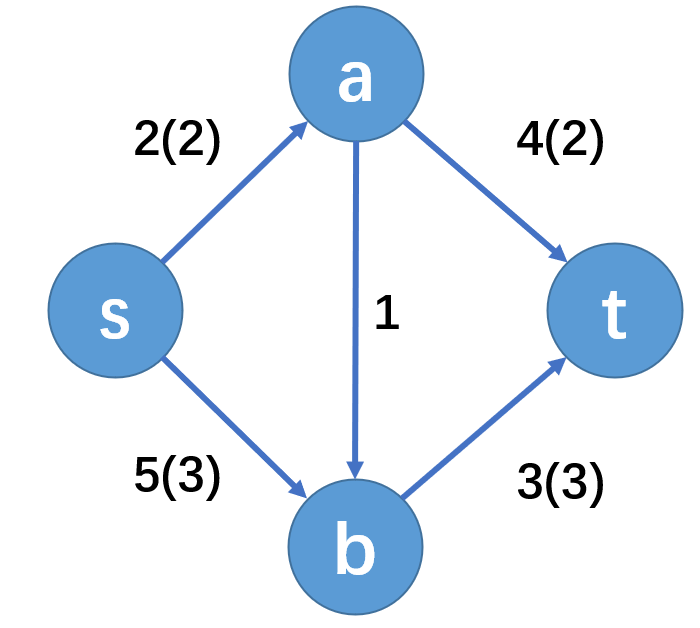
\includegraphics[scale=0.25]{P4.png}
        \caption{Flow Graph of Step 2}
    \end{figure}
    \begin{figure}[H]
        \centering
        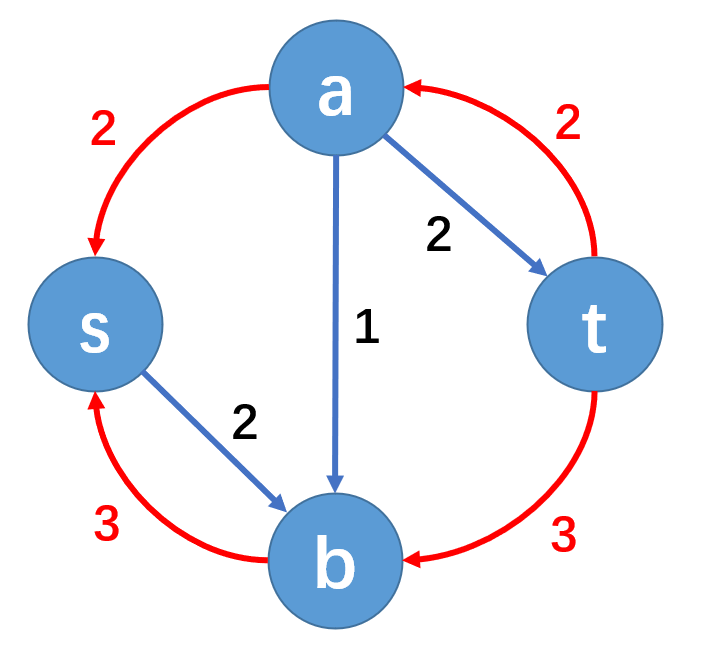
\includegraphics[scale=0.25]{P5.png}
        \caption{Residual Graph of Step 2}
    \end{figure}
    Since there is no more path $p\rightarrow t$, the max flow is 5
\end{enumerate}
\textbf{Task 2}
Yes, because by looking the original graph intuitively, we can easily find the max flow is 2000, and the algorithm only needs to take two steps if it prefers $s\rightarrow a\rightarrow t$ and $s\rightarrow b\rightarrow t$
\begin{figure}[H]
    \centering
    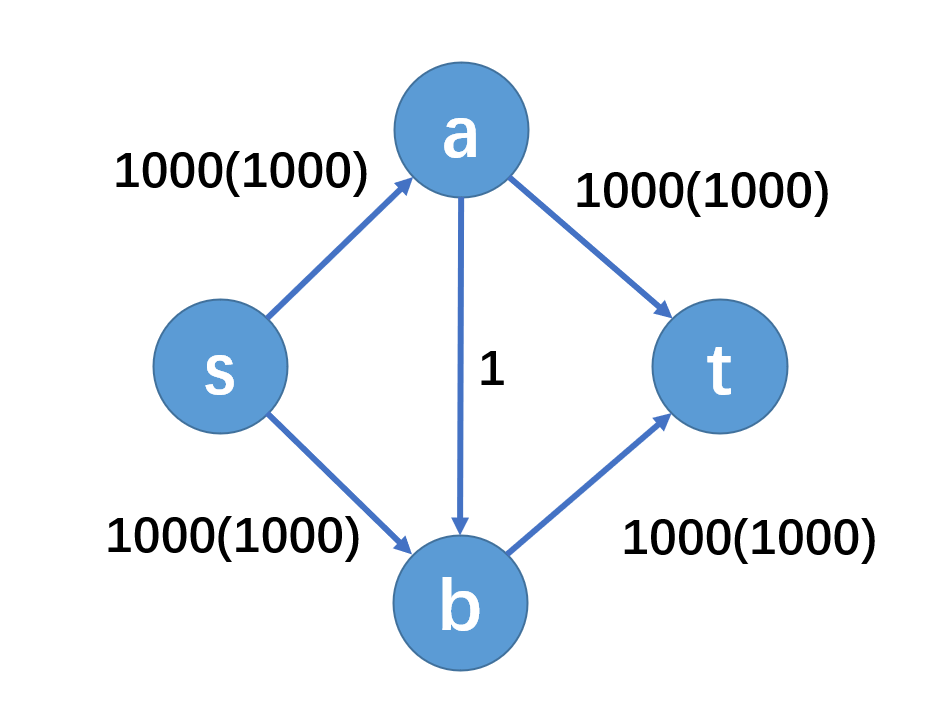
\includegraphics[scale=0.25]{P6.png}
    \caption{Intuitive Path}
\end{figure}
However, if the algorithm prefers $E_{ab}$, the first path will either be $s\rightarrow a\rightarrow t$ or $s\rightarrow b\rightarrow t$ with flow 1. 
\begin{figure}[H]
    \centering
    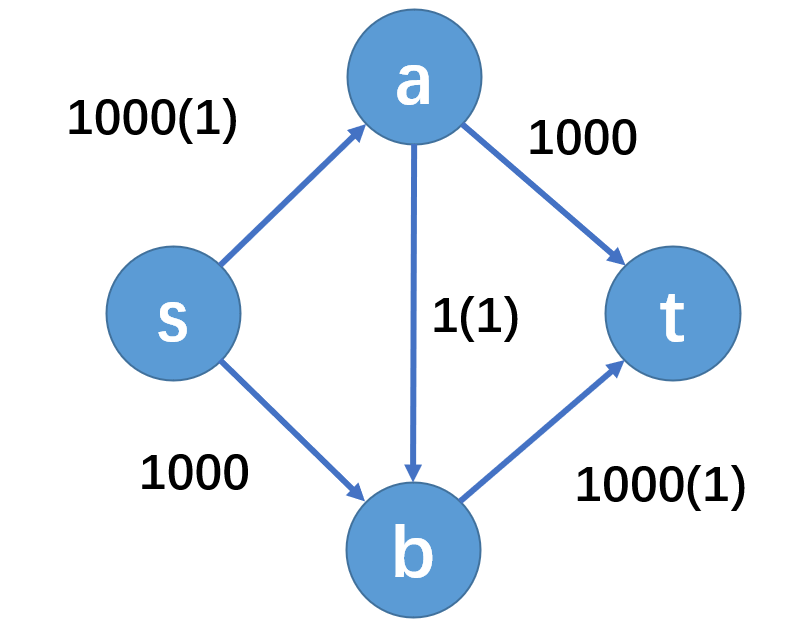
\includegraphics[scale=0.25]{P7.png}
    \caption{Flow Graph of Step 1}
\end{figure}
\begin{figure}[H]
    \centering
    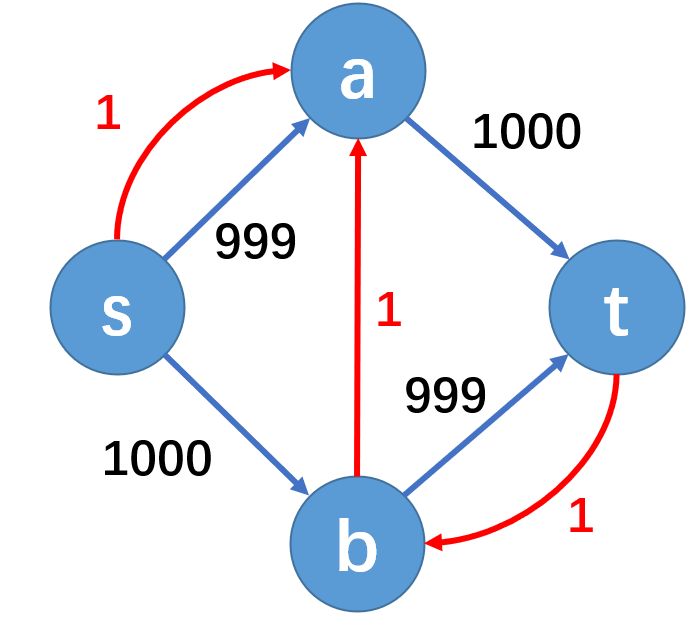
\includegraphics[scale=0.25]{P8.png}
    \caption{Residual Graph of Step 1}
\end{figure}
Then, according to the perference and residual graph, the next path will be the opposite one, but still with flow 1. Therefore, it takes 2000 steps for the algorithm to find the max flow. So the perference to $E{ab}$ will lead to more steps for the algorithm.
\section*{Python Code}
\begin{verbatim}
import numpy as np
import pandas as pd
from gurobipy import *
import matplotlib.pyplot as plt

df = pd.DataFrame(pd.read_csv(r"D:\PANDA\Study\VG441\Homework\Problem Set 2\demand.csv"))
d = df.d_t.T
T, K, h = 52, 1100, 2.4
M = 10e5
# 导入数据
WW = Model()
q = WW.addVars(T, lb=np.zeros(T), vtype=GRB.CONTINUOUS, name="order_quantity")
x = WW.addVars(T, lb=np.zeros(T), vtype=GRB.CONTINUOUS, name="inventory_level")
y = WW.addVars(T, vtype=GRB.BINARY, name="if_order")

WW.setObjective(quicksum(K*y[t]+h*x[t] for t in range(T)), GRB.MINIMIZE)

c1 = WW.addConstrs(q[t] <= M*y[t] for t in range(T))
c2 = WW.addConstrs(x[t] == x[t-1] + q[t] - d[t] for t in range(1,T))
c3 = WW.addConstr(x[0] == q[0] - d[0])
WW.optimize()
# WW.printAttr('X')
print(WW.getAttr('X',q).values())

t=np.linspace(0,T-1,T)
X=[234.9999999999999, 122.99999999999835, 0.0, 297.0, 150.0, 0.0, 174.0, 0.0, 197.0, 0.0, 206.99999999999997, 0.0, 240.00000000000006, 0.0, 241.0000000000011, 0.0, 267.0, 0.0, 289.9999999999999, 0.0, 301.0, 1.4203321069368455e-12, 324.9999999999985, 0.0, 343.0000000000001, 0.0, 340.0, 0.0, 323.0, 0.0, 309.0, 0.0, 293.0, 0.0, 272.9999999999999, 0.0, 248.99999999999994, 0.0, 234.99999999999994, 0.0, 204.0, 0.0, 182.99999999999994, 0.0, 163.99999999999994, 0.0, 299.0, 145.0, 0.0, 224.0, 112.0, 0.0]

Q=[342.9999999999999, 0.0, 1.2505552149377763e-12, 426.0000000000004, 0.0, 0.0, 330.0, 0.0, 386.0, 0.0, 409.0, 0.0, 468.00000000000006, 0.0, 483.00000000000216, 0.0, 533.0, 0.0, 559.9999999999999, 0.0, 604.0, 1.4203321069368455e-12, 653.9999999999972, 1.553065288008162e-12, 688.0000000000001, 0.0, 707.0, 0.0, 660.0, 0.0, 634.0, 0.0, 598.0, 0.0, 545.9999999999999, 0.0, 500.99999999999994, 0.0, 477.99999999999994, 0.0, 430.0, 0.0, 386.99999999999994, 0.0, 338.99999999999994, 0.0, 461.0, 0.0, 0.0, 361.0, 0.0, 0.0]
plt.plot(t,X,color='blue',label='Inventory Level')
plt.plot(t,Q,color='red',label='Order Quantity')
plt.plot(t,d,color='green',label='Demand')
plt.legend(loc='upper left', fontsize=10)
plt.show()
\end{verbatim}
\end{document}